% !TeX spellcheck = el_GR-en_US
  \documentclass[11pt]{article}
  \usepackage{geometry}
  \geometry{a4paper, top=2.5cm, bottom=2.5cm, left=2.2cm,
    right=2.2cm}
  \usepackage{fontspec}
  \usepackage[nonumeralsign]{xgreek}
  \usepackage{fancyhdr}
  \usepackage{hyperref}
  \usepackage{enumitem}
  \usepackage{cite}
  \usepackage{multirow}
  \usepackage{graphicx}

  \setmainfont{Baskerville}
  \setmonofont{Consolas}

  \graphicspath{ {./images/} }
  
  \newcommand{\ypertitlos}{Εργασία στο μάθημα Βάσεις Δεδομένων}
  \newcommand{\titlos}{AwesomenameDB}
  \newcommand{\ypotitlos}{Βάση δεδομένων για εκδηλώσεις στην πόλη}
  \newcommand{\paradoteo}{1ο Παραδοτέο}
  \newcommand{\omada}{Ομάδα 19 αν θυμάμαι καλά...}
  \newcommand{\student}[3]{#1&#2&#3\\}
  \newcommand{\melosA}{\student{Μπλάννινγκ
      Φρανκ}{6689}{frankgou@auth.gr}}
  \newcommand{\melosB}{\student{Θεοδωρίδου Χριστίνα}{8055}{}}
  \newcommand{\melosC}{\student{Ζησης Μηλης Εμμανουηλ}{8053}{}}
  \newcommand{\hmnia}{\today}
  
  \pagestyle{fancy}
  \lhead{Βάσεις Δεδομένων 2018}
  \rhead{\titlos}
  \renewcommand{\headrulewidth}{0.4pt}
  \renewcommand{\footrulewidth}{0.4pt}
  \setlength{\headheight}{14pt}

  \hypersetup{colorlinks=true, linkcolor=black, urlcolor=blue, citecolor=blue}
  \urlstyle{same}

  \begin{document}
  \thispagestyle{empty}
  {\centering
    \Large\ypertitlos\\
    \vspace{7cm}
    \Huge\titlos\\
    \Large\ypotitlos\\
    \vspace{2cm}
  }
  \hfill \paradoteo
  
  \vspace{8cm}
  \begin{tabular}[b]{l l l}
    \omada&&\\
    \melosA
    \melosB
    \melosC
  \end{tabular}
  
  {\centering
    \vspace{2cm}
    \hmnia\\
  }
  \newpage

  \tableofcontents
  \listoffigures

  \newpage
  
  \section{Εισαγωγή}

\subsection{Σκοπός Εφαρμογής}

Οι σύγχρονες πόλεις, καθημερινά, δίνουν την δυνατότητα σε πολλούς
καλλιτέχνες και μη, να προβάλουν την δουλειά τους μέσω εκθέσεων,
συναυλιών ή άλλων εκδηλώσεων. Επίσης, καθημερινά διάφοροι οργανισμοί
και ομάδες διοργανώνουν διάφορες δραστηριότητες προς υποστήριξη και
ενημέρωση του κόσμου για τον σκοπό τους.

Αποτέλεσμα όλων αυτών είναι, στην σημερινή κοινωνία, τα δρώμενα που
λαμβάνουν χώρα καθημερινά να είναι πολυπληθή. Έτσι είναι απαραίτητη
μια εφαρμογή όπου θα περιέχει πληροφορίες για όλες αυτές τις
εκδηλώσεις έτσι ώστε να μπορούν οι ενδιαφερόμενοι να βρίσκουν τις
δραστηριότητες που τους ενδιαφέρουν. Μία τέτοια εφαρμογή απαιτεί μία
βάση δεδομένων για την αποθήκευση, προσπέλαση και επεξεργασία των
Πληροφοριών κάθε εκδήλωσης λόγο του μεγάλου όγκου της πληροφορίας
αυτής και την ανάγκη για παράλληλη επεξεργασία δεδομένων από πολλούς
χρήστες.

\subsection{Περιγραφή Εφαρμογής}

Συγκεκριμένα, στη δική μας εφαρμογή, εκος από τοποθεσία, είδος και
ημερομηνία της εκδήλωσης, ο χρήστης θα μπορεί να αγοράσει εισιτήρια
εκδηλώσεων ή να βρει φυσικά καταστήματα προπώλησης, να αποθηκεύσει
εκδηλώσεις που τον ενδιαφέρουν ώστε να τις δει αργότερα και άλλα. Όλα
αυτά είναι εφικτά λόγο της προσεκτικής σχεδίασης της βάσης δεδομένων
πίσω από την εφαρμογή

Για την βάση \titlos, τα δεδομένα, που θα αποθηκεύονται είναι το όνομα
των εκδηλώσεων, το είδος τους, οι ημερομηνίες διεξαγωγής τους, η
τοποθεσία που πραγματοποιούνται κτλ. Τη βάση θα μπορεί αν την
χρησιμοποιήσει ο οποιοσδήποτε, αρκεί να έχει πρόσβαση σε αυτήν μέσω
του διαδικτύου, στον ιστότοπο στον οποίο θα βρίσκεται. Επίσης, όποιος
θα ήθελε η εκδήλωσή του να δημοσιοποιηθεί, θα μπορεί συμπληρώνοντας
μια φόρμα εγγραφής να αποκτήσει πρόσβασή στην πλατφόρμα δημιουργίας
εκδήλωσης και να προστεθεί η εκδήλωση του στον ιστότοπο.

\subsection{Απαιτήσεις Εφαρμογής σε Δεδομένα}

Για την βάση \titlos, αναμένεται να έχουμε ~1050 κωδικούς εκδηλώσεων
(πχ για έναν μήνα) , που σημαίνει ~35 κωδικοί εκδηλώσεων κάθε
μέρα. Επίσης, αναμένεται οι ~20 να είναι μουσικής, οι ~25 να είναι
κάτα μέσο όρο απογευματινές ώρες κτλ



%%% Local Variables:
%%% mode: latex
%%% TeX-master: "main"
%%% End:

  
\section{Κατηγορίες Χρηστών και απαιτήσεις τους}

Στην συγκεκριμένη εφαρμογή και κατ' επέκταση η βάση δεδομένων θα έχει
έναν διαχειριστή και τρεις χρήστες, τον "Διοργανωτή" τον "Μη
Εγγεγραμμένο Χρήστη" και τον "Χρήστη". Μόνο οι τρεις χρήστες ορίζονται
παρακάτω μιας και ο διαχειριστής της εφαρμογής και της βάσης δεδομένων
θα εκτελεί ενέργειες με αυτόνομο τρόπο πέρα των πλαισίων της
εφαρμογής.

\underline{Διοργανωτής:}

Ο Διοργανωτής, μετά από εγγραφή του στο σύστημα, η οποία εγκρίνεται
από τον διαχειριστή, πρέπει να έχει την δυνατότητα να εκτελεί όλες τις
απαραίτητες ενέργειες έτσι ώστε να καταχωρεί όλες τις απαραίτητες
πληροφορίες μιας εκδήλωσης όπως και να έχει πρόσβαση στην λίστα αγορών
για τις εκδηλώσεις όπου διαχειρίζεται. Αναλυτικά:
\begin{itemize}[noitemsep]
\item Προσθήκη νέας τοποθεσίας διεξαγωγής
\item Προσθήκη νέων σημείων προπόλησης
\item Προσθηκη νέας εκδήλωσης
\item Προβολή λίστας αγορών εκδήλωσης όπου οργανώνει
\end{itemize}

\underline{Μη εγγεγραμμένος χρήστης}

Ο μη εγγεγραμμένος χρήστης έχει την δυνατότητα να προβάλει με διάφορα
κριτήρια εύρεσης τις μελλοντικές εκδηλώσεις και να πραγματοποιήσει
εγγραφή
\begin{itemize}[noitemsep]
\item Πρόσβαση σε δεδομένα που αφορούν τις εκδηλώσεις, μετά απο
  σχετική αναζήτηση.
\item Εγγραφή χρήστη
\end{itemize}

\underline{Χρήστης:}

Ο Χρήστης μετά από εγγραφή του, η οποία ολοκληρώνεται αυτόματα, έχει
την επιπλέον δυνατότητα, πέρα του μη εγγεγραμμένου χρήστη, να εκτελεί
αγορά εισιτήριων για τις εκδηλώσεις που το υποστηρίζουν, όπως και να
αποθηκεύει εκδηλώσεις που των ενδιαφέρουν για να τις δει
αργότερα. Αναλυτικά:
\begin{itemize}[noitemsep]
\item Προσθήκη νέας κάρτας πληρωμής
\item Αγορά εισιτήριου εκδήλωσης
\item Προσθήκη και αφαίρεση εκδήλωσης στην λίστα ενδιαφερομένων
\item Προβολή εκδηλώσεων στην λίστα ενδιαφερομένων
\end{itemize}


%%% Local Variables:
%%% mode: latex
%%% TeX-master: "main"
%%% End:

  \section{Μοντέλο Οντοτήτων/Συσχετίσεων}

\subsection{Γενική Περιγραφή}

Οι οντότητες είναι : οι Εκδήλωση, η Τοποθεσία, η Ημερομηνία, ο Καλλιτέχνης - Διοργανωτής, η Αγορά Εισιτηρίων και η Προσβασιμότητα. Για κάθε εκδήλωση θα πρέεπι να καταγράφεται το όνομά της, το είδος της και το όνομα του καλλιτέχνη-διοργανωτή.
\\
\\
\underline{Υποθέσεις:}
\begin{itemize}[noitemsep]

\item Ο κωδικός εκδήλωσης είναι μοναδικός για κάθε εκδήλωση. Για παράδειγμα, εφόσον ο κωδικός 101 αντιστοιχεί σε μια συγκικριμένη εκδήλωση (ασχέτως καλλιτέχνη ή τοποθεσίας), την ημερομηνία 1/12/2018, τότε ο ίδιος κωδικός δεν μπορεί να είναι κωδικός καμίας άλλης εκδήλωσης.
\item Η διαφημίσεις μπορούν να γίνουν μόνο σε έναν τηλεοπτικό ή ραδιοφωνικό σταθμό για κάθε εκδήλωση. Επίσης θα υπάρχει μόνο ένα μέρος τοποθέτησης αφισών κάθε φορά.


\end{itemize}

\subsection{Καθορισμός Οντοτήτων}

Παρακάτω φαίνονται οι οντότητες της \titlos, η περιγραφή τους καθώς και κάποια γνωρίσματά τους.

\begin{center}
\begin{tabular}[]{|c | c|}
\hline
\textbf{Όνομα Οντότητας}   &  Event  \\ \hline 
\textbf{Περιγραφή}         &  Οντότητα που αποθηκεύονται οι εκδηλώσεις \\ \hline 
\textbf{Ιδιότητες}         &  Ισχυρή οντότητα \\  \hline               
\textbf{Γνωρίσματα}        &  \underline{Κωδικός εκδήλωσης} \\
           ~               &  Είδος εκδήλωσης \\
            ~              &  Ύπαρξη Εισιτηρίου \\
             ~             &  Κοινό που απευθύνεται \\
              ~            &  Σκοπός \\ 
                           &  Ημερομηνία \\
                           &  Ώρα \\
\hline
\hline
\textbf{Όνομα Οντότητας}   &  Location \\ \hline 
\textbf{Περιγραφή}         &  Οντότητα που αποθηκεύονται οι τοποθεσίες των εκδηλώσεων \\ \hline 
\textbf{Ιδιότητες}         &  Ασθενής οντότητα \\ \hline 
\textbf{Γνωρίσματα}        &  \underline{Κωδικός τοποθεσίας} \\
                           &  Όνομα \\
           ~               &  Οδός \\
             ~             &  ΤΚ\\
                           &  Εσωτερικός ή Εξωτερικός χώρος \\
                           &  Τηλέφωνο \\
                           & { \begin{tabular}[]{c|c}
                            Κάτάλογος τιμών           & μπύρα \\
                                                      & κρασί \\
                                                      & ποτό \\  
                           \end{tabular} }  
\\ \hline

\end{tabular}

\begin{tabular}[]{|c | c | } 
\hline
\textbf{Όνομα Οντότητας}   &  Artist \\ \hline 
\textbf{Περιγραφή}         &  Οντότητα που αποθηκεύονται οι καλλιτέχνες \\ \hline 
\textbf{Ιδιότητες}         &  Ισχυρή οντότητα    \\    \hline           
\textbf{Γνωρίσματα}        &  \underline{Κωδικός καλλιτέχνη}\\
                           &  Όνομα Καλλιτέχνη \\
           ~               &  Καταγωγή \\
            ~              &  Είδος \\
\hline 
\hline
\textbf{Όνομα Οντότητας}   &  Tickets \\ \hline 
\textbf{Περιγραφή}         &  Οντότητα που αποθηκεύονται οι τρόποι αγοράς εισιτηρίων \\\hline 
\textbf{Ιδιότητες}         &  Ασθενής οντότητα \\       \hline           
\textbf{Γνωρίσματα}        &  \underline{Κωδικός εκδήλωσης} \\
                          %  &  Ύπαρξη εισιτηρίου \\
                           &  Φυσικά καταστήματα προπώλησης \\
           ~               &  Ηλεκτρονικά καταστήματα προπώλησης \\
            ~              &  Εύρος τιμών \\
\hline 
\hline
\textbf{Όνομα Οντότητας}   &  Accessibility \\ \hline 
\textbf{Περιγραφή}         &  Οντότητα που αποθηκεύονται οι τρόποι πρόσβασης στην τοποθεσια \\ \hline 
\textbf{Ιδιότητες}         &  Ασθενής οντότητα \\  \hline                 
\textbf{Γνωρίσματα}        &  \underline{Κωδικός Τοποθεσίας} \\
                           &  Ύπαρξη χώρου στάθμευσης\\
            ~              &  Ύπαρξη κοντινών στάσεων \\
             ~             &  Ύπαρξη υποδομών για ΑΜΕΑ \\
                           & { \begin{tabular}[]{c|c}
                             Ύπαρξη τοποθεσιών με μισθωμένα ΜΜΜ           & τοποθεσία \\
                                                                         & ώρα \\ 
                           \end{tabular} }  
\\ \hline
\hline
\textbf{Όνομα Οντότητας}   &  Promotion \\ \hline 
\textbf{Περιγραφή}         &  Οντότητα που αποθηκεύονται οι τρόποι προώθησης της εκδήλωσης \\ \hline 
\textbf{Ιδιότητες}         &  Ασθενής οντότητα \\  \hline                 
\textbf{Γνωρίσματα}        &  \underline{Κωδικός Εκδήλωσης} \\
                           &  Ραδιοφωνικοί σταθμοί \\
            ~              &  Τηλεοπτικοί σταθμοί \\
             ~             &  Τοποθεσίες αφισών \\
                           & { \begin{tabular}[]{c|c}
                             Διαδικτυακή διαφήμηση & Κοινωνικά δίκτυα \\
                                                   & Ψηφιακές εφημερίδες \\
                                                   & Διάφορες ιστοσελίδες\\ 
                           \end{tabular} }  
\\ \hline
\hline
\textbf{Όνομα Οντότητας}   &  Communication \\ \hline 
\textbf{Περιγραφή}         &  Οντότητα που αποθηκεύονται οι τρόποι επικοινωνίας \\ \hline 
\textbf{Ιδιότητες}         &  Ασθενής οντότητα \\  \hline                 
\textbf{Γνωρίσματα}        &  \underline{Κωδικός Εκδήλωσης} \\
                           &  \underline{Όνομα Καλλιτέχνη} \\
            ~              &  Όνομα εταιρίας παραγωγής \\
             ~             &  email \\
                           &  Τηλέφωνο \\
\\ \hline
\end{tabular}
\end{center}


\subsection{Καθορισμός Συσχετίσεων}

Παρακάτω αναφέρονται οι συσχετίσεις της βάσης δεδομένων \titlos

\begin{tabular}[]{|p{4cm}|p{10cm}|}
  \hline
  \textbf{Όνομα Συσχέτισης} & Event\_Has\_Artist\\ \hline
  \textbf{Περιγραφή} & Κάθε εκδήλωση πρέπει να έχει 1 καλλιτέχνη\\ \hline
  \textbf{Ιδιότητες} & Has-A \{αναφέρετε αν είναι Is-A και αν είναι
                       Αναδρομική, Προσδιορίζουσα, Τριαδική\} \\ \hline
  \textbf{Λόγος πληθικότητας} & n:1 \\ \hline
  \textbf{Συμμετοχή} & Ολική Συμμετοχή του Event \\ \cline{2-2}
                     & Μερική Συμμετοχή του Artist \\ \hline
  \textbf{Γνωρίσματα} & - \\ \hline
\end{tabular}


\begin{tabular}[]{|p{4cm}|p{10cm}|}
  \hline
  \textbf{Όνομα Συσχέτισης} & Event\_Has\_Location\\ \hline
  \textbf{Περιγραφή} & Κάθε εκδήλωση πρέπει να έχει 1 τοποθεσία\\ \hline
  \textbf{Ιδιότητες} & Has-A \{αναφέρετε αν είναι Is-A και αν είναι
                       Αναδρομική, Προσδιορίζουσα, Τριαδική\} \\ \hline
  \textbf{Λόγος πληθικότητας} & n:1 \\ \hline
  \textbf{Συμμετοχή} & Ολική Συμμετοχή του Event \\ \cline{2-2}
                     & Μερική Συμμετοχή του Location \\ \hline
  \textbf{Γνωρίσματα} & - \\ \hline
\end{tabular}


\begin{tabular}[]{|p{4cm}|p{10cm}|}
  \hline
  \textbf{Όνομα Συσχέτισης} & Event\_Has\_Date\\ \hline
  \textbf{Περιγραφή} & Κάθε εκδήλωση πρέπει να έχει 1 ημερομηνία\\ \hline
  \textbf{Ιδιότητες} & Has-A \{αναφέρετε αν είναι Is-A και αν είναι
                       Αναδρομική, Προσδιορίζουσα, Τριαδική\} \\ \hline
  \textbf{Λόγος πληθικότητας} & n:1 \\ \hline
  \textbf{Συμμετοχή} & Ολική Συμμετοχή του Event \\ \cline{2-2}
                     & Μερική Συμμετοχή του Date \\ \hline
  \textbf{Γνωρίσματα} & - \\ \hline
\end{tabular}


\begin{tabular}[]{|p{4cm}|p{10cm}|}
  \hline
  \textbf{Όνομα Συσχέτισης} & Event\_Has\_Date\\ \hline
  \textbf{Περιγραφή} & Κάθε εκδήλωση πρέπει να έχει 1 ημερομηνία\\ \hline
  \textbf{Ιδιότητες} & Has-A \{αναφέρετε αν είναι Is-A και αν είναι
                       Αναδρομική, Προσδιορίζουσα, Τριαδική\} \\ \hline
  \textbf{Λόγος πληθικότητας} & n:1 \\ \hline
  \textbf{Συμμετοχή} & Ολική Συμμετοχή του Event \\ \cline{2-2}
                     & Μερική Συμμετοχή του Date \\ \hline
  \textbf{Γνωρίσματα} & - \\ \hline
\end{tabular}

\begin{tabular}[]{|p{4cm}|p{10cm}|}
  \hline
  \textbf{Όνομα Συσχέτισης} & Event\_Has\_Tickets\\ \hline
  \textbf{Περιγραφή} & Κάθε εκδήλωση πρέπει να έχει μέρη που πωλούνται εισιτήρια\\ \hline
  \textbf{Ιδιότητες} & Has-A \{αναφέρετε αν είναι Is-A και αν είναι
                       Αναδρομική, Προσδιορίζουσα, Τριαδική\} \\ \hline
  \textbf{Λόγος πληθικότητας} & n:1 \\ \hline
  \textbf{Συμμετοχή} & Ολική Συμμετοχή του Event \\ \cline{2-2}
                     & Μερική Συμμετοχή του Tickets\\ \hline
  \textbf{Γνωρίσματα} & - \\ \hline
\end{tabular}

\begin{tabular}[]{|p{4cm}|p{10cm}|}
  \hline
  \textbf{Όνομα Συσχέτισης} & Location\_Has\_Accessibility\\ \hline
  \textbf{Περιγραφή} & Κάθε τοποθεσία πρέπει να έχει τρόπους πρόσβασης\\ \hline
  \textbf{Ιδιότητες} & Has-A \{αναφέρετε αν είναι Is-A και αν είναι
                       Αναδρομική, Προσδιορίζουσα, Τριαδική\} \\ \hline
  \textbf{Λόγος πληθικότητας} & n:1 \\ \hline
  \textbf{Συμμετοχή} & Ολική Συμμετοχή του Location \\ \cline{2-2}
                     & Μερική Συμμετοχή του Accessibility\\ \hline
  \textbf{Γνωρίσματα} & - \\ \hline
\end{tabular}

\begin{tabular}[]{|p{4cm}|p{10cm}|}
  \hline
  \textbf{Όνομα Συσχέτισης} & Event\_Has\_Communication\\ \hline
  \textbf{Περιγραφή} & Κάθε εκδήλωση πρέπει να έχει τρόπους επικοινωνίας\\ \hline
  \textbf{Ιδιότητες} & Has-A \{αναφέρετε αν είναι Is-A και αν είναι
                       Αναδρομική, Προσδιορίζουσα, Τριαδική\} \\ \hline
  \textbf{Λόγος πληθικότητας} & n:n \\ \hline
  \textbf{Συμμετοχή} & Ολική Συμμετοχή του Event \\ \cline{2-2}
                     & Μερική Συμμετοχή του Communication \\ \hline
  \textbf{Γνωρίσματα} & - \\ \hline
\end{tabular}

\begin{tabular}[]{|p{4cm}|p{10cm}|}
  \hline
  \textbf{Όνομα Συσχέτισης} & Event\_Has\_Promotion\\ \hline
  \textbf{Περιγραφή} & Κάθε εκδήλωση πρέπει να έχει τρόπους προώθησης\\ \hline
  \textbf{Ιδιότητες} & Has-A \{αναφέρετε αν είναι Is-A και αν είναι
                       Αναδρομική, Προσδιορίζουσα, Τριαδική\} \\ \hline
  \textbf{Λόγος πληθικότητας} & n:n \\ \hline
  \textbf{Συμμετοχή} & Ολική Συμμετοχή του Event \\ \cline{2-2}
                     & Μερική Συμμετοχή του Promotion \\ \hline
  \textbf{Γνωρίσματα} & - \\ \hline
\end{tabular}

\subsection{Διάγραμμα Οντοτήτων/Συσχετίσεων}

\{Δείξτε το διάγραμμα Ο/Σ για τη βάση. Το διάγραμμα μπορείτε να το
κατασκευάσετε σε πρόγραμμα της επιλογής σας, ωστόσο θα πρέπει να
ακολουθεί το συμβολισμό Chen (δηλαδή οντότητες ως παραλληλόγραμμα,
συσχετίσεις ως ρόμβοι, διπλή γραμμή για υποχρεωτική συμμετοχή, κτλ.)\}

Παράδειγμα για τη FlightsDB:
\begin{figure}[H]
  \centering
  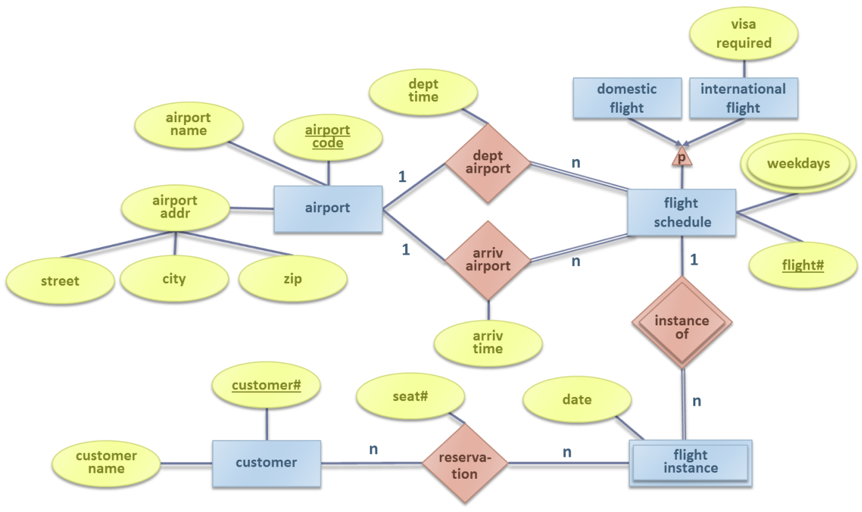
\includegraphics[width=\linewidth]{entities.png}
  \caption{Διάγραμμα Οντοτήτων/Συσχετίσεων}
\end{figure}


%%% Local Variables:
%%% mode: latex
%%% TeX-master: "main"
%%% End:

  % \input{2.past_implementations.tex}
  % \input{3.our_implementation.tex}

  % \bibliographystyle{ieeetr}
  % \bibliography{cites}{}
  % \bibliographystyle{plain}

\end{document}